\documentclass{article}

\usepackage[french]{babel}
\usepackage[utf8]{inputenc}
\usepackage{graphicx}
\usepackage{amsmath, amssymb}
\usepackage{geometry}
\usepackage{algorithm2e}
\usepackage{enumerate,enumitem}
\usepackage{caption}
\usepackage{subcaption}
\usepackage{url}
\usepackage{hyperref}

%%%%%%%%%%%%%%%% Lengths %%%%%%%%%%%%%%%%
\setlength{\textwidth}{15.5cm}
\setlength{\evensidemargin}{0.5cm}
\setlength{\oddsidemargin}{0.5cm}

%%%%%%%%%%%%%%%% Variables %%%%%%%%%%%%%%%%
\def\projet{1}
\def\titre{M\'ethodes de calcul numérique/Limites de la machine}
\def\groupe{4}
\def\equipe{18224}
\def\responsible{gardouin}
\def\secretary{mhajjilaamo}
\def\others{electakone, hbastien, acattarin}

\begin{document}

%%%%%%%%%%%%%%%% Header %%%%%%%%%%%%%%%%
\noindent\begin{minipage}{0.98\textwidth}
  \vskip 0mm
  \noindent
  { \begin{tabular}{p{7.5cm}}
      {\bfseries \sffamily
        Projet \projet} \\ 
      {\itshape \titre}
    \end{tabular}}
  \hfill 
  \fbox{\begin{tabular}{l}
      {~\hfill \bfseries \sffamily Groupe \groupe\ - Equipe \equipe
        \hfill~} \\[2mm] 
      Responsable : \responsible \\
      Secrétaire : \secretary \\
      Codeurs : \others
    \end{tabular}}
  \vskip 4mm ~


 %%%%%%%%%%%%%%%%%%%%%%%%%%%%%%%%%%%%%%%%%%%%%%%%%%%%%%%%%%%%%%%%%%% Présentation du travail
   ~~~\parbox{0.95\textwidth}{\small \textit{Résumé~:} \sffamily Ce projet consiste à l’application de méthodes de calcul numérique et aux limitations que l'on rencontre. La première partie met en évidence des exemples dans lesquels les opérations élémentaires ne sont pas assez précises, tandis que la seconde partie s'intéresse à l'approximation du logarithme népérien et aux algorithmes CORDIC utilisés dans les calculatrices de poche.}
  \vskip 1mm ~

  %%%%%%%%%%%%%%%%%%%%%%%%%%%% motivation du projet
  %%%%%%%%%%%%%%%%%%%%%%%%%%%% lien avec le cours

Ce projet est en lien direct avec le cours d'IS104 dans lequel nous nous sommes intéressés aux méthodes de calcul numérique. Il permet notamment d'illustrer les limitations que l'on peut rencontrer.

  %%%%%%%%%%%%%%%%%%%%%%%%%%%% part du projet réalisée
  % Non nécessaire : projet réalisé en intégralité
\end{minipage}

  
%%%%%%%%%%%%%%%% Main part %%%%%%%%%%%%%%%%
\section{Représentation des nombres en machine}
\label{sec:repr_nb_machine}

%%%%%%%%%%%%%%%%%%%%%%%%%%%%%%%%%%%%%%%%%%%%%%%%%%%%%%%%%%%%%%%%%%%%%%%% Code

%%%%%%%%%%%%%%%%%%%%%%%%%%%%%%%%%%%%%%%%%%%%%%%%%%%%%%%%%%%%%%%% chapeau d'introduction de la partie 1

\textit{Dans cette partie, nous allons utiliser Python pour réaliser des simulations de représentation des nombres en machine. En particulier, nous définirons une fonction permettant d'obtenir la représentation décimale réduite d'un réel et nous nous appuierons sur cette fonction pour simuler les opérations d'addition et de multiplication sur machine.}
\vskip 1mm ~

  %%%%%%%%%%%%%%%%%%%%%%%%%%%%%%%%%%%%%%%%%%%%%%%%%%%%%%%%%%%%%%% Partie 1


  %%%%%%%%%%%%%%%%%%%%%%%%%%%%%%%%% repésentation décimale réduite
 
Tout d'abord, nous avons implémenté en Python une fonction \verb|rp(x,p)| permettant d'obtenir la représentation décimale réduite d'un réel $x$. La variable $p$ désigne la précision des décimales.

Cette fonction commence par écrire $x$ sous son écriture scientifique, réalise ensuite un arrondi à $p-1$ décimales et repasse enfin $x$ dans son écriture standard.

Le jeu de valeurs représenté en figure~\ref{fig:tests_rp} permet d'illustrer le fonctionnement de cette fonction. Nous nous sommes également servi de ces valeurs afin de vérifier le bon fonctionnement de la fonction.

\begin{figure}[h]
  \centering
  \begin{tabular}{|l|l|l|}
    \hline
    $x$ & $\texttt{rp(x,4)}$ & $\texttt{rp(x,6)}$ \\
    \hline
    $3,141592658$ & $3,142$ & $3,14159$ \\
    \hline
    $10507,1823$ & $10510$ & $10507,2$ \\
    \hline
    $0,0001857563$ & $0,0001858$ & $0,000185756$ \\
    \hline
  \end{tabular}
   \caption{Jeu de valeurs servant aux tests de la fonction \texttt{rp(x,p)}}
   \label{fig:tests_rp}
\end{figure}

Le passage en écriture scientifique est une opération de complexité temporelle d'ordre $O(\log(x))$. Le passage inverse est de coût constant car on garde en mémoire la puissance de $10$ de l'écriture scientifique. L'opération d'arrondi est considérée comme constante. Ainsi, la complexité temporelle de \verb|rp(x,p)| est de l'ordre de $O(\log(x))$.
\vskip 1mm ~

  %%%%%%%%%%%%%%%%%%%%%% description

  %%%%%%%%% nom de la fonction

  %%%%%%%%% définition de chacune des variables

  %%%%%%%%% exemples démontrant le bon fonctionnement du code (repésentation graphique si possible)
  
  %%%%%%%%%%%%%%% Si fonction principale

  %%%%%%%%%% Estimation de la complexité

  %%%%%%%%%% évaluation du comportement dans les cas limites




  %%%%%%%%%%%%%%%%%%%%%%%%%%%%%%%%% addition et multiplication en représation décimale réduite
 
À partir de cette fonction, nous avons pu réaliser des fonctions d'addition et de multiplication qui s'appuyent sur la représentation décimale réduite.

Ces fonctions sont \verb|add(x1,x2)| et \verb|mult(x1,x2)| et réalisent respectivement l'addition et la multiplication des représentations décimales de \verb|x1| et \verb|x2| à la précision $p=3$. Nous réalisons ces opérations à l'aide de la fonction \verb|rp(x,p)|.
\vskip 1mm ~

  %%%%%%%%%%%%%%%%%%%%%% description

  %%%%%%%%% nom de la fonction

  %%%%%%%%% définition de chacune des variables

  %%%%%%%%% exemples démontrant le bon fonctionnement du code (repésentation graphique si possible)
  
  %%%%%%%%%%%%%%% Si fonction principale

  %%%%%%%%%% Estimation de la complexité

  %%%%%%%%%% évaluation du comportement dans les cas limites


  
  %%%%%%%%%%%%%%%%%%%%%%%%%%%%%%%%% erreur relative réalisée en ajoutant y à x
 
Enfin, à l'aide des fonctions \verb|add(x1,x2)| et \verb|mult(x1,x2)|, nous avons pu étudier les erreurs relatives de ces opérations en implémentant deux nouvelles fonctions, \verb|delta_add(x,y)| et \verb|delta_mult(x,y)|. Les opérations réalisées par ces deux fonctions sont représentées par les équation~\ref{eq:delta_add} et~\ref{eq:delta_mult}.

\begin{equation}
  \texttt{delta\_add(x,y)} = \dfrac{\big\vert x + y - \texttt{add(x,y)} \big\vert}{\big\vert x+y \big\vert}
  \label{eq:delta_add}
\end{equation}

\begin{equation}
  \texttt{delta\_mult(x,y)} = \dfrac{\big\vert x \times y - \texttt{mult(x,y)} \big\vert}{\big\vert x\times y \big\vert}
  \label{eq:delta_mult}
\end{equation}
À l'aide de ces fonctions, nous pouvons réaliser l'étude des erreurs relatives pour un $x$ fixé. Voir fin du document pour les graphes des tests réalisés. Ces erreurs relatives sont représentées en figure~\ref{fig:relative_error}.

\begin{figure}[ht]
  \centering
  \begin{subfigure}[b]{0.5\textwidth}
    \centering
    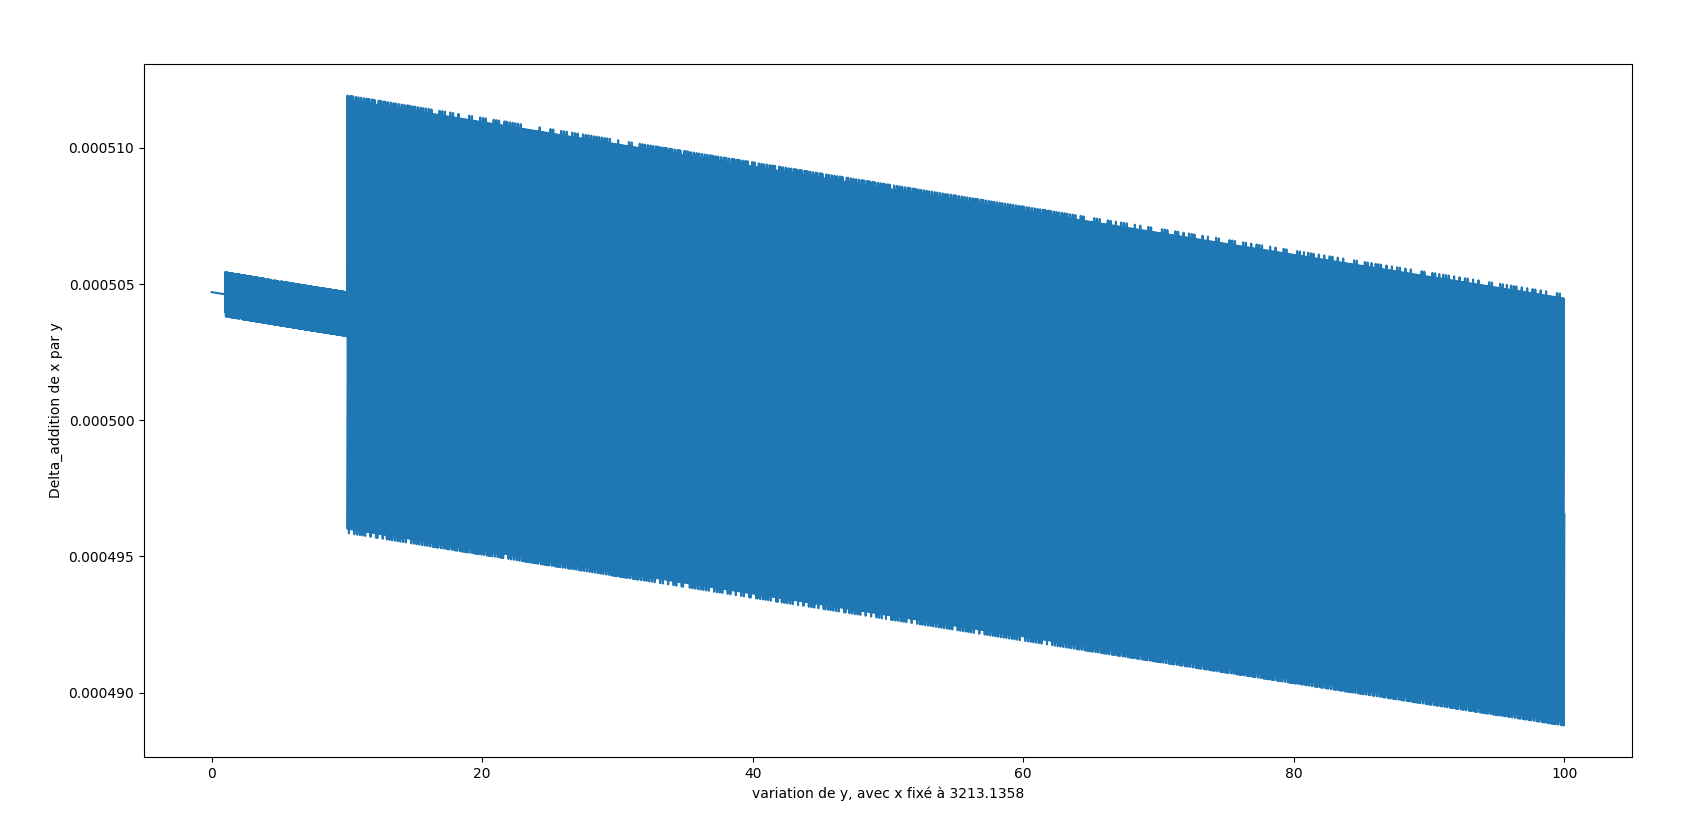
\includegraphics[width=\linewidth]{Partie1-delta_add_0-100.png}
    \caption{Erreur relative pour l'addition de $x = ????$ et $y\in[0,100]$}
    \label{subfig:delta_add_big}
  \end{subfigure}
  \hfill
  \begin{subfigure}[b]{0.5\textwidth}
    \centering
    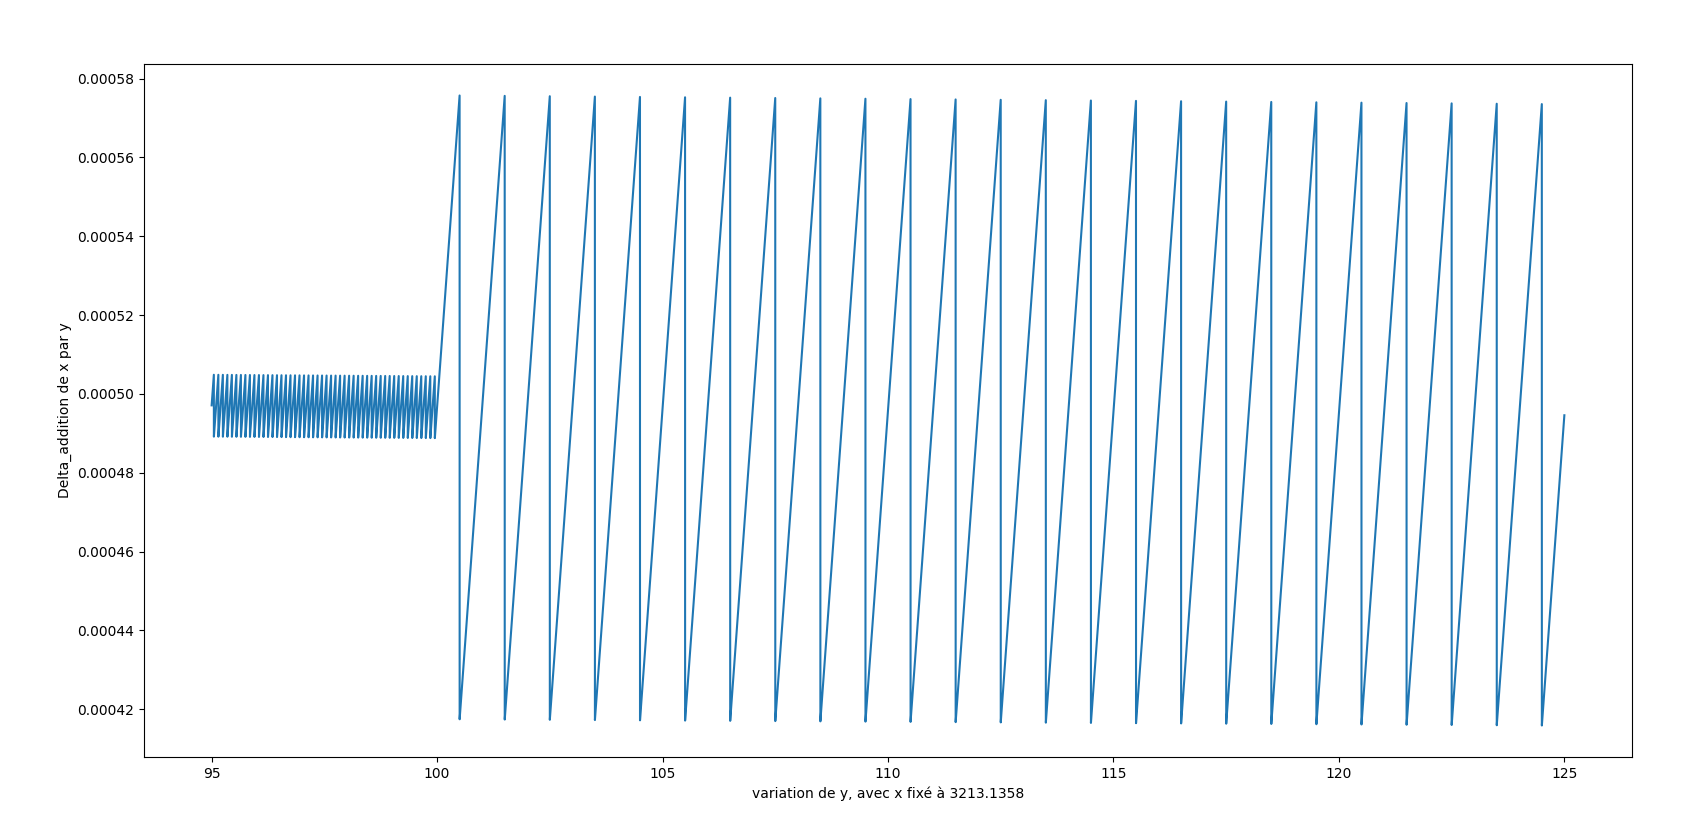
\includegraphics[width=\linewidth]{Partie1-delta_add_95-125.png}
    \caption{Erreur relative pour l'addition de $x = ????$ et $y\in[95,125]$}
    \label{subfig:delta_add_zoom}
  \end{subfigure}
  \begin{subfigure}[b]{0.5\textwidth}
    \centering
      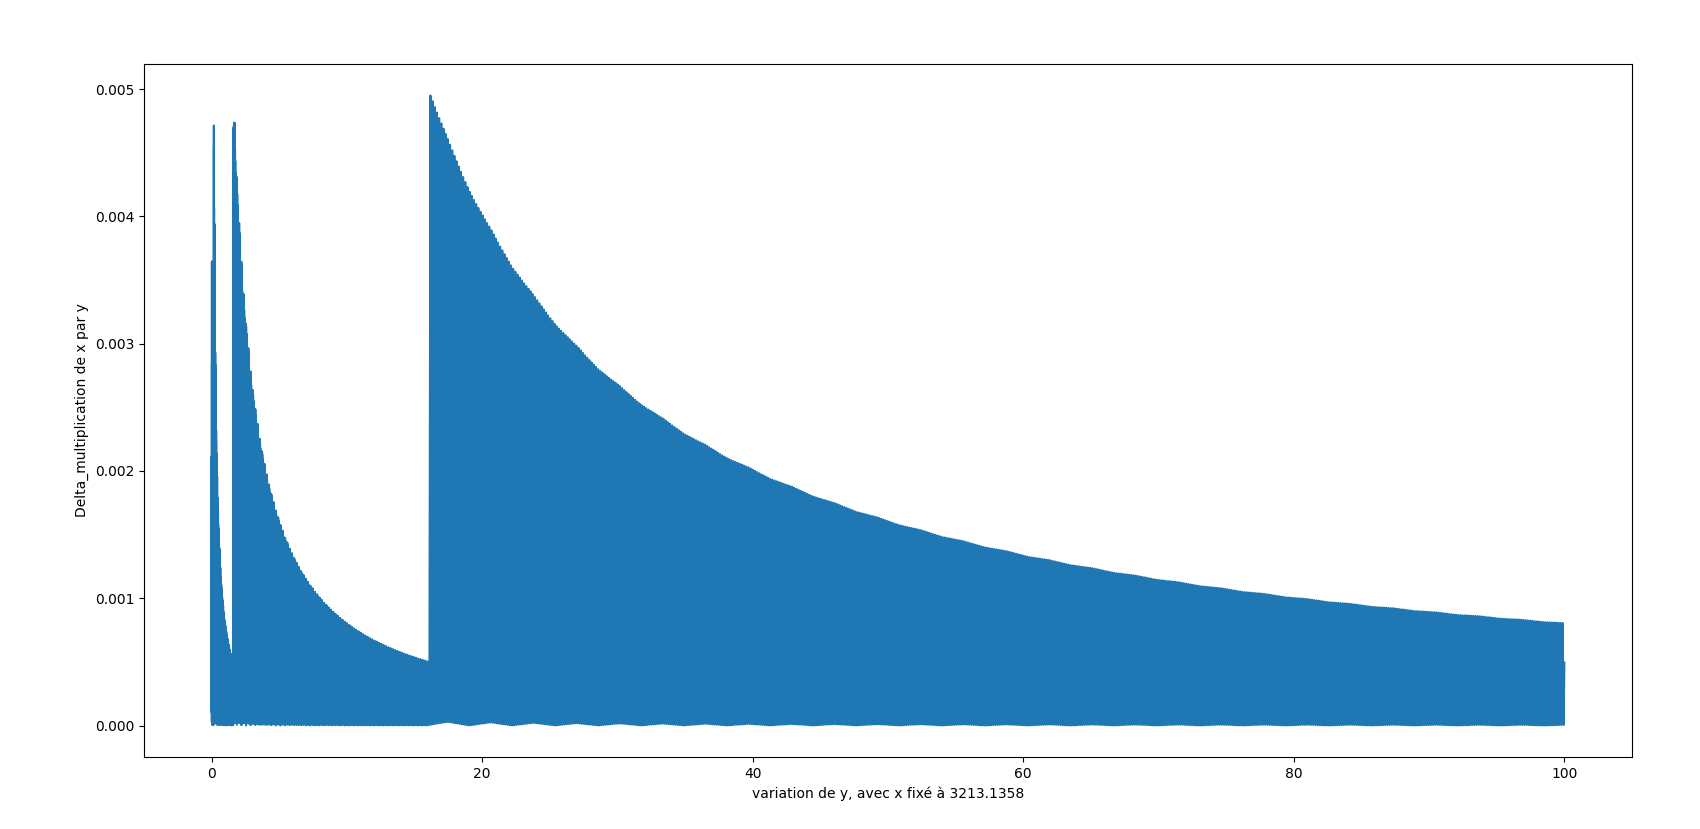
\includegraphics[width=\linewidth]{Partie1-delta_mult_0-100.png}
      \caption{Erreur relative pour la multiplication de $x = ????$ et $y\in[0,100]$}
      \label{subfig:delta_multi_big}
  \end{subfigure}
  \begin{subfigure}[b]{0.5\textwidth}
    \centering
    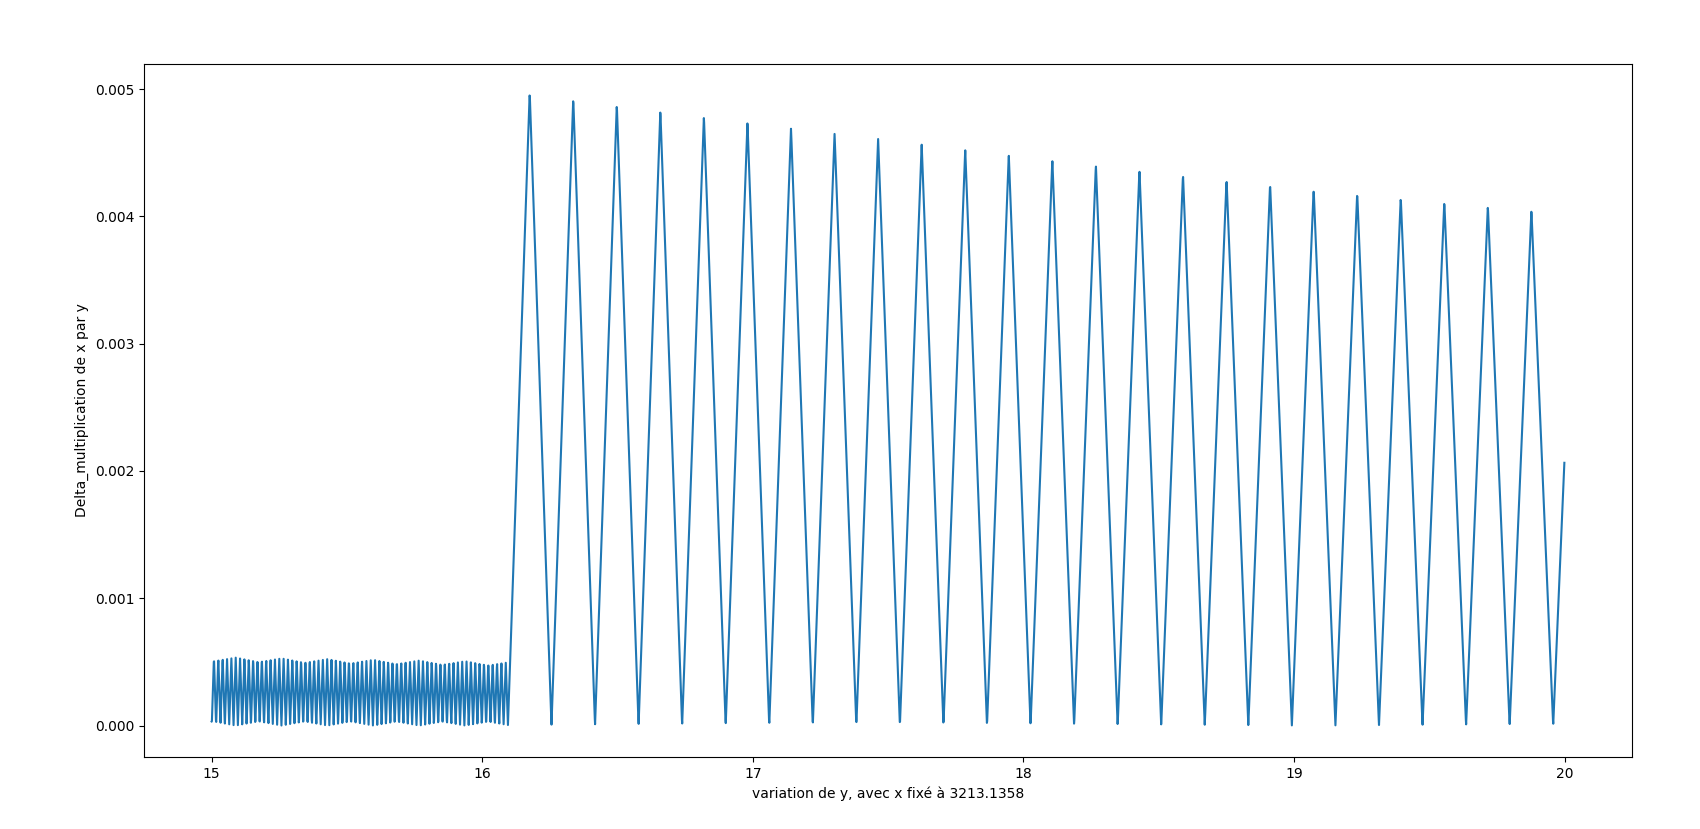
\includegraphics[width=\linewidth]{Partie1-delta_mult_15-20.png}
    \caption{Erreur relative pour la multiplication de $x = ????$ et $y\in[15,20]$}
    \label{subfig:delta_mult_zoom}
    \end{subfigure}
  \caption{Représentations des erreurs relatives pour l'addition et la multiplication}
  \label{fig:relative_error}
\end{figure}

[COMMENTAIRES AVEC RÉFÉRENCES]



%\begin{figure}[ht]
%  \centering
%  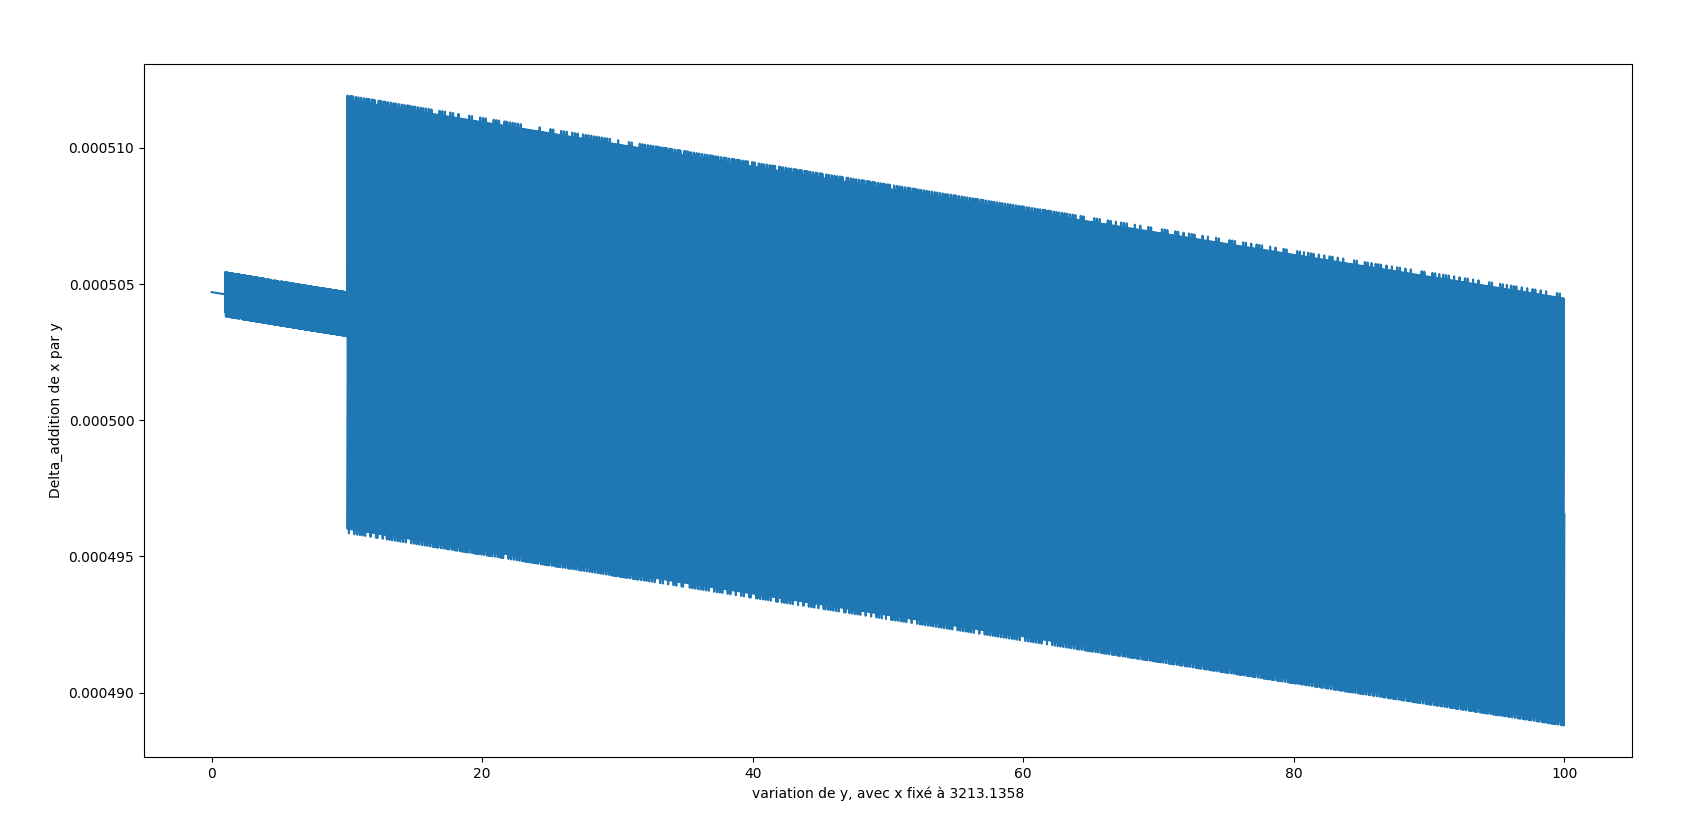
\includegraphics[width=0.5\textwidth]{Partie1-delta_add_0-100.png}
%  \caption{...}
%  \label{fig:delta_add_big}        
%\end{figure}

%\begin{figure}[ht]
%  \centering
%  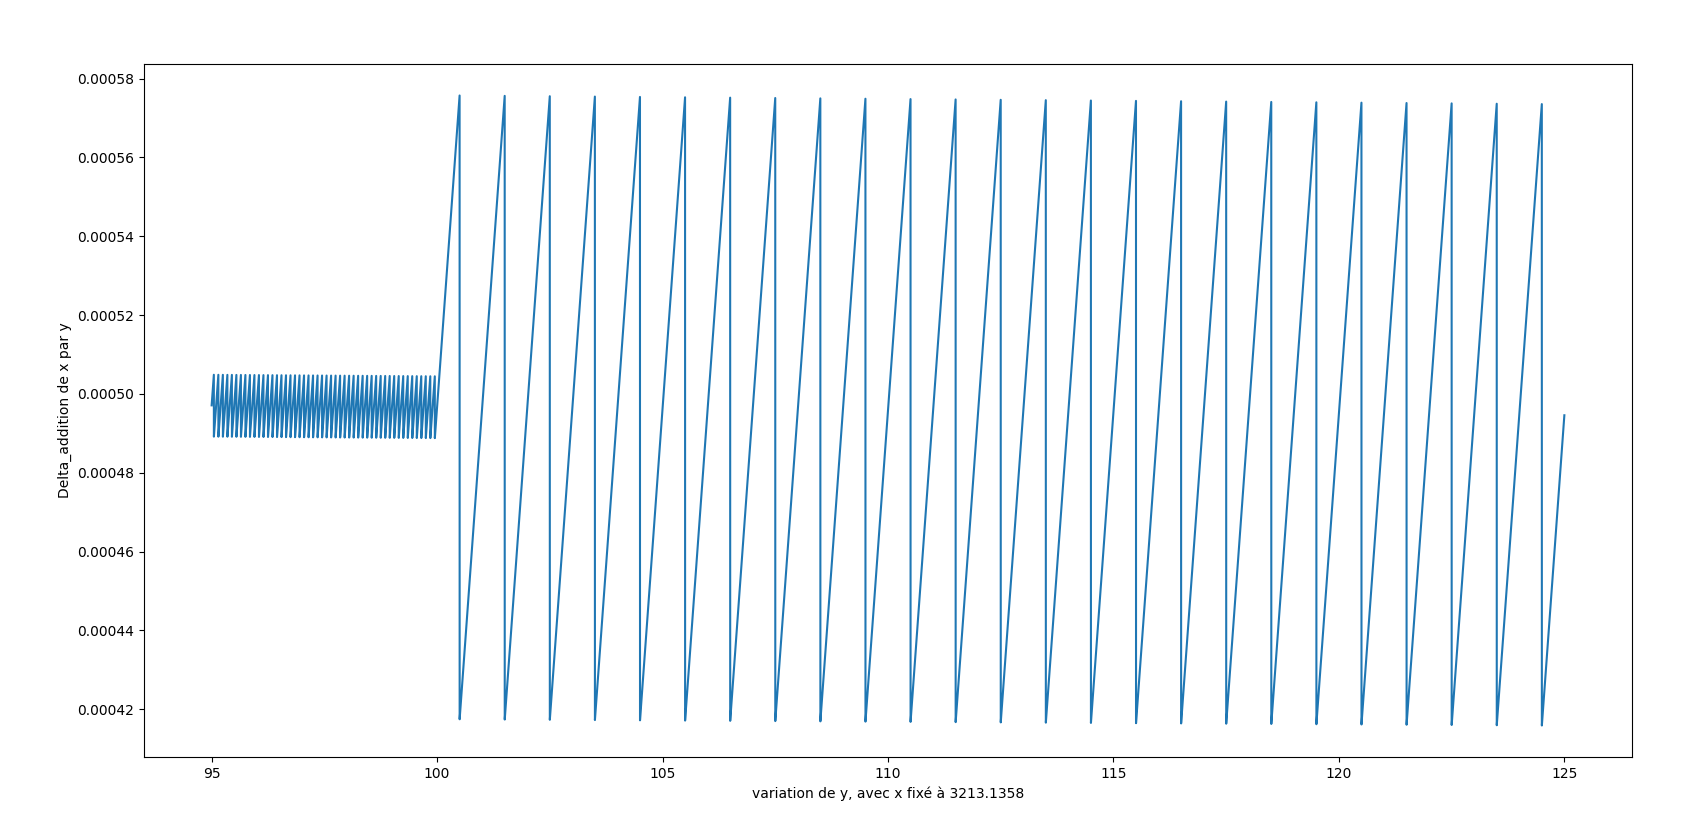
\includegraphics[width=0.5\textwidth]{Partie1-delta_add_95-125.png}
%  \caption{...}
%  \label{fig:delta_add_zoom}        
%\end{figure}

%\begin{figure}[ht]
%  \centering
%  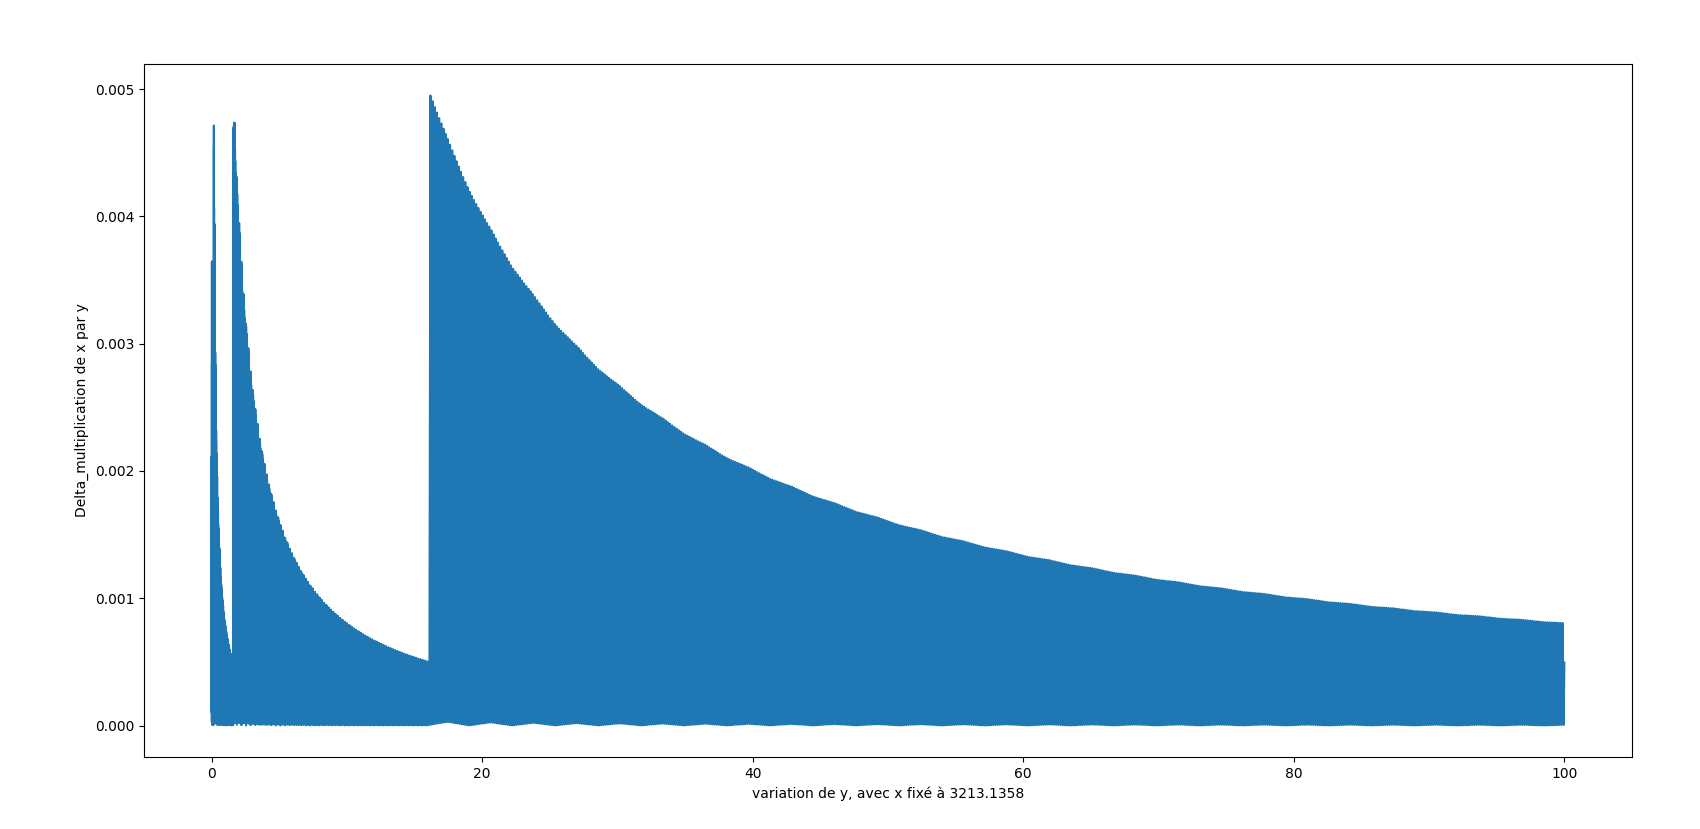
\includegraphics[width=0.5\textwidth]{Partie1-delta_mult_0-100.png}
%  \caption{...}
%  \label{fig:delta_mult_big}        
%\end{figure}

%\begin{figure}[ht]
  %\centering
  %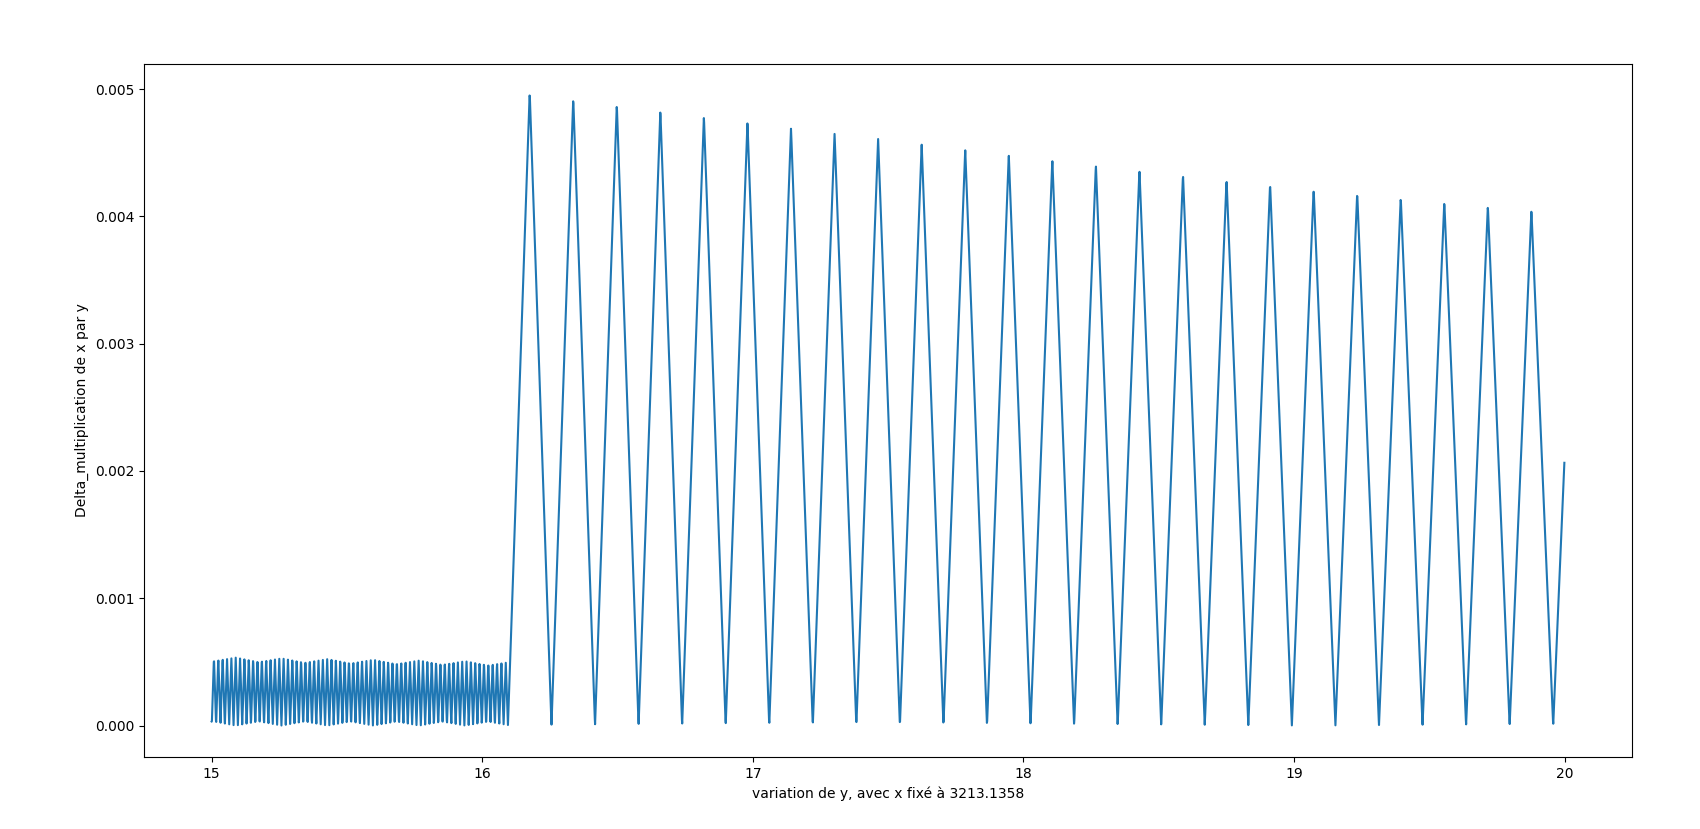
\includegraphics[width=0.5\textwidth]{Partie1-delta_mult_15-20.png}
  %\caption{...}
 % \label{fig:delta_mult_zoom}        
%\end{figure}
 
  %%%%%%%%%%%%%%%%%%%%%% description

  %%%%%%%%% nom de la fonction

  %%%%%%%%% définition de chacune des variables

  %%%%%%%%% exemples démontrant le bon fonctionnement du code (repésentation graphique si possible)
  
  %%%%%%%%%%%%%%% Si fonction principale

  %%%%%%%%%% Estimation de la complexité

  %%%%%%%%%% évaluation du comportement dans les cas limites


  
  %%%%%%%%%%%%%%%%%%%%%%%%%%%%%%%%% erreur relative réalisée en multipliant x et y
 
  %%%%%%%%%%%%%%%%%%%%%% description

  %%%%%%%%% nom de la fonction

  %%%%%%%%% définition de chacune des variables

  %%%%%%%%% exemples démontrant le bon fonctionnement du code (repésentation graphique si possible)
  
  %%%%%%%%%%%%%%% Si fonction principale

  %%%%%%%%%% Estimation de la complexité

  %%%%%%%%%% évaluation du comportement dans les cas limites


  
  %%%%%%%%%%%%%%%%%%%%%%%%%%%%%%%%% graphe des fonctions précédentes
 
  %%%%%%%%%%%%%%%%%%%%%% description

  %%%%%%%%% nom de la fonction

  %%%%%%%%% définition de chacune des variables

  %%%%%%%%% exemples démontrant le bon fonctionnement du code (repésentation graphique si possible)
  
  %%%%%%%%%%%%%%% Si fonction principale

  %%%%%%%%%% Estimation de la complexité

  %%%%%%%%%% évaluation du comportement dans les cas limites

\section{Logarithme népérien de 2}
\label{sec:ln}
%%%%%%%%%%%%%%%%%%%%%%%%%%%%%%%%%%%%%%%%%%%%%%%%%%%%%%%%%%%%%%%% chapeau d'introduction de la partie 2
\textit{Il s'agit ici de mettre en application la partie 1 en calculant une valeur approchée de $\log(2)$ sur p d\'ecimales, tout en \'evaluant l'erreur relative obtenue.}
\vskip 1mm ~

Nous avons commencé par réaliser l'implémentation de l'algorithme~\ref{alg:algo_ln} en Python.

\begin{algorithm}
  \caption{Calcul d'une valeur approchée de $\log(2)$ sur p d\'ecimales}
  \label{alg:algo_ln}
  \KwData{int $p$}
  \KwResult{$log(2)$}
  $res \gets 0$\;
  $i \gets 1$\;
  \While{$i<10^6$}{
    \eIf{$i$ is even}{
      $res \gets res - \frac{1}{i}$\;
    }{$res \gets res + \frac{1}{i}$\;}
    $i \gets i + 1$\;
  }
  Return $\texttt{rp(}res,p\texttt{)}$\;
\end{algorithm}


%%%[ erreur relative ?  ]%%%[ commentaire ]


Afin d'estimer l'erreur relative commise par la fonction \verb|calc_log|, nous avons implémenté, avec une fonction \verb|delta_log|, le calcul présenté par l'équation~\ref{eq:delta_log}.

\begin{equation}
  \texttt{delta\_log(p)} = \dfrac{\big\vert \log(2) - \texttt{calc\_log(p)} \big\vert}{\big\vert \log(2) \big\vert}
  \label{eq:delta_log}
 \end{equation} 

La figure~\ref{fig:relative_error_log} illustre cette erreur relative pour des valeurs de $p$ allant de $1$ à $20$. On peut remarquer que l'erreur est relativement importante pour $p<3$, mais que au-delà de $p=5$, l'erreur se stabilise environ à $2.10^{-5}$, ce qui représente une erreur acceptable.

\begin{figure}[ht]
 \centering
 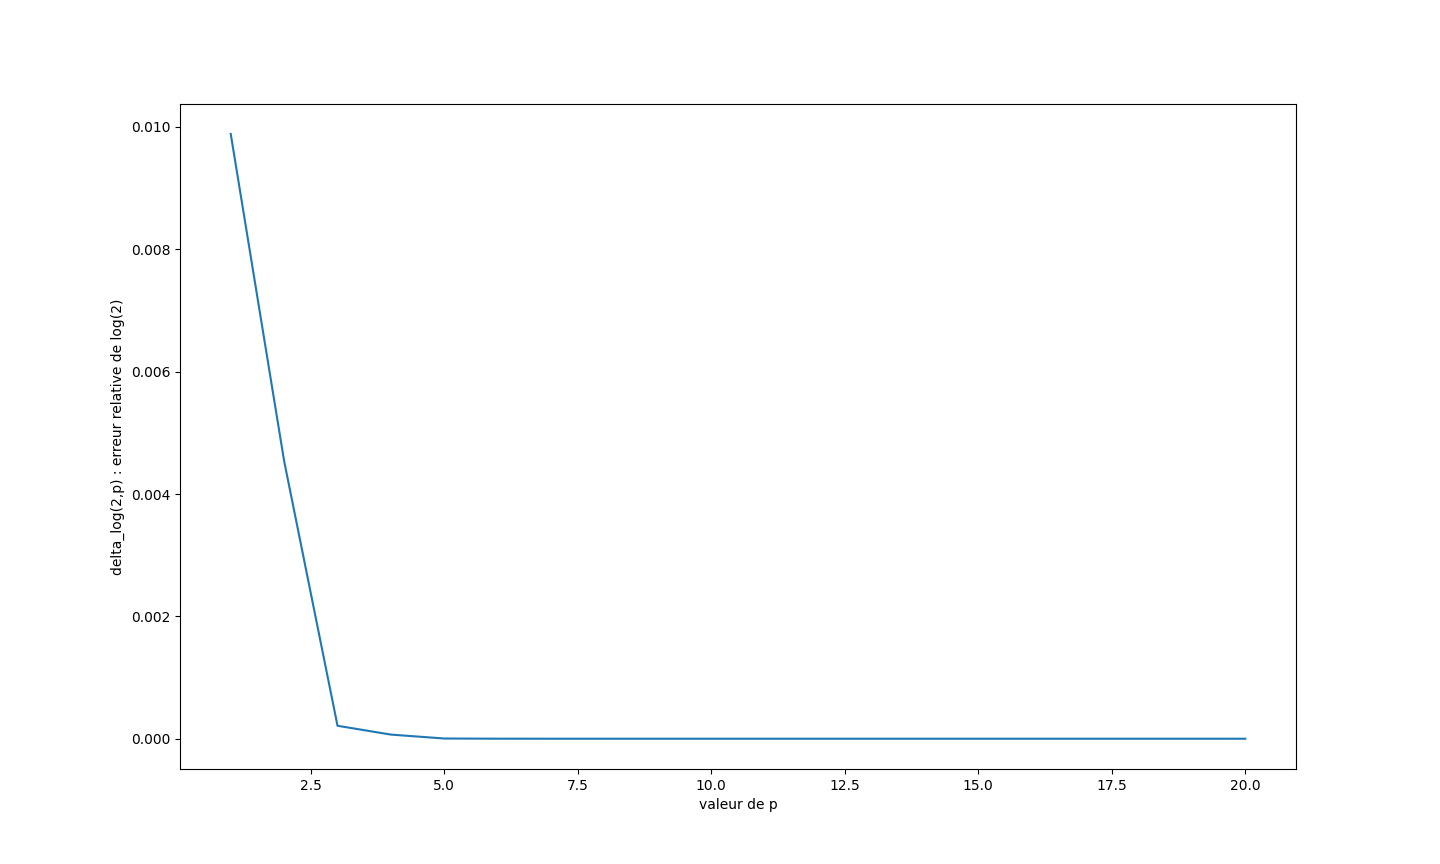
\includegraphics[width=0.8\textwidth]{partie2_relative_error_log.png}
 \caption{Erreur relative de la fonction $\texttt{calc\_log}$ pour différentes valeurs de $p$}
 \label{fig:relative_error_log}        
\end{figure}


  %%%%%%%%%%%%%%%%%%%%%%%%%%%%%%%%%%%%%%%%%%%%%%%%%%%%%%%%%%%%%%% Partie 2


  %%%%%%%%%%%%%%%%%%%%%%%%%%%%%%%%% Logarithme népérien de 2
 
  %%%%%%%%%%%%%%%%%%%%%% description

  %%%%%%%%% nom de la fonction

  %%%%%%%%% définition de chacune des variables

  %%%%%%%%% exemples démontrant le bon fonctionnement du code (repésentation graphique si possible)
  
  %%%%%%%%%%%%%%% Si fonction principale

  %%%%%%%%%% Estimation de la complexité

  %%%%%%%%%% évaluation du comportement dans les cas limites


\section{Algorithmes CORDIC}
\label{sec:cordic}
  %%%%%%%%%%%%%%%%%%%%%%%%%%%%%%%%% algorithmes CORDIC

\textit{Les ressources disponibles en m\'emoire ou en puissance de calcul sont en g\'en\'eral limit\'ees. Il devient donc n\'ecessaire de disposer d'algorithmes qui permettent de contourner ces limitations tout en conservant des résultats de calculs satisfaisants. Dans cette section, on s'int\'eresse à l'exemple d'une calculatrice typique.}
\vskip 1mm ~


  %%%%%%%%%%%%%%%%%%%%%% Calculatrice
  %%%%%%%%%%% référence

{\small \textit{\textbf{N.B:}} \emph{ Les réponses ci-dessous sont en partie inspirée du chapitre VI.2 de la FAQ\footnote{\url{http://www.usenet-fr.net/fur/maths/maths-faq-3.html}} du groupe de discussions fr.sci.maths\footnote{\url{https://groups.google.com/g/fr.sci.maths}}}.
  \vskip 0.01mm ~
 
  %%%%%%%%% représentation des nombres utilisés sur une calculatrice
  Dans une calculatrice typique un nombre 'flottant' occupe 8 octets de m\'emoire et est d\'ecompos\'e en:
  \begin{itemize}
     \item une mantisse de 13 chiffres cod\'es ind\'ependamment sur 4 chiffres binaires (Binaire Code Decimal ou BCD)
     \item un exposant (puissance de 10) \'eventuellement sign\'e
     \item le signe du nombre (et de l'exposant s'il n'est pas sign\'e)
  \end{itemize}

  
  %%%%%%%%% avantages et inconvénients de ce genre de représentation
  Ceci a l'avantage de permettre la r\'ealisation d'op\'erations complexes avec du mat\'eriel plus ou moins minimal. De plus, le calcul de toute fonction standard est ramen\'e au calcul des quatre fonctions : ln, exp, tan et arctan. Cela est cependant conditionn\'e par la donnée de certaines valeurs pr\'ecalcul\'ees, ce qui peut \^etre consid\'er\'e comme un inconv\'enient. D'autre part, l'efficacit\'e des algorithmes diminue en augmentant la valeur des nombres calcul\'es.

  \vskip 1mm ~

  %%%%%%%%%%%%%%%%%%%%%%% algorithmes pour calculer les fonctions exp et trigonométriques

  Maintenant, nous voulons trouver un moyen pour évaluer les fonctions exponentielle et trigonométriques. Concr\'etement, plusieurs techniques se pr\'esentent pour r\'ealiser cette t\^ache. En particulier, on s'int\'eresse aux algorithmes CORDIC (Coordinate Rotation Digital Computer) sur les calculatrices, introduient dans la m\^eme section qu'évoquée en début de section~\ref{sec:cordic}. La technique de base nécessite une valeur pr\'ecalcul\'ee (par exemple $\ln(10)$ pour le calcul de la fonction $\ln$) et se d\'eroule en deux \'etapes :
  \begin{enumerate}
  \item Ramener la valeur à \'evaluer dans l'intervalle où la m\'ethode est applicable. Voici un exemple de transformation utilis\'ee pour le calcul de la fonction $\ln$ sur $[1,10[$ :
      \begin{equation}
        \ln(x) = \ln(x*10^{-n}) + n*\ln(10)
      \end{equation}
    \item Appliquer l'algorithme correspondant en int\'erant sur l'indice k de l'\'el\'ement pr\'ecalcul\'e en commen\c cant par le plus grand terme.
  \end{enumerate}
  Cette m\'ethode est bien adapt\'ee aux conditions impos\'ees par une calculatrice, entre autres : une m\'emoire et une puissance de calcul limit\'ee.
  %%%%%%%%% technique générale utilisée

  %%%%%%%%% efficacité lorsqu'elle est ramenée à une calculatrice


  
  %%%%%%%%%%%%%%%%% implémentation des quatres algorithmes

  
  %%%%%%%%%%%% exp et ln
 
  %%%%%%%%%%%%%%%% description

  %%%%%%%%% nom de la fonction

  %%%%%%%%% définition de chacune des variables

  %%%%%%%%% exemples démontrant le bon fonctionnement du code (repésentation graphique si possible)
  
  %%%%%%%%%%%%%%% Si fonction principale

  %%%%%%%%%% Estimation de la complexité

  %%%%%%%%%% évaluation du comportement dans les cas limites


  
  %%%%%%%%%%%%%%%% tan et arctan
 
  %%%%%%%%%%%%%%%%%%%%%% description

  %%%%%%%%% nom de la fonction

  %%%%%%%%% définition de chacune des variables

  %%%%%%%%% exemples démontrant le bon fonctionnement du code (repésentation graphique si possible)
  
  %%%%%%%%%%%%%%% Si fonction principale

  %%%%%%%%%% Estimation de la complexité

  %%%%%%%%%% évaluation du comportement dans les cas limites



  %%%%%%%%%%%%%%%%%%%%% vérification des algorithmes par la méthode ?


%%%%%%%%%%%%%%%%%%%%%%%%%%%%%%%%%%%%%%%%%%%%%%%%%%%%%%%%%%%%%%%%%% conclusion

  %%%%%%%%%%%%%%%%%%%%%%%%%%% commentaire <participant>



  %%%%%%%%%%%%%%%%%%%%%%%%%%% commentaire <participant>


  
  %%%%%%%%%%%%%%%%%%%%%%%%%%% commentaire <participant>



  %%%%%%%%%%%%%%%%%%%%%%%%%%% commentaire <participant>



  %%%%%%%%%%%%%%%%%%%%%%%%%%% commentaire <participant>

  
  


\end{document}
